\chapter{Visual Studio Code extension}
\label{chap:VS_code_extension}
\textbf{Author:} Florian Prandstetter

\section{Introduction}

This chapter provides an overview of the VS Code extension developed for the project. It describes its core functionality, and explains how it integrates with the broader system architecture.

\section{What is VS Code}

VS Code is a free code editor from Microsoft. It supports many programming languages such as Python, JavaScript, and C++.

A major advantage of VS Code is its extensibility. With extensions, you can customize the editor, for example, with debugging tools, themes, or special functions for specific programming languages. It also offers features like auto-completion, integrated Git support, and a built-in terminal function.

VS Code is lightweight and runs on Windows, macOS, and Linux. Despite this, it provides many features that are also found in a full-fledged integrated development environment. This makes it perfect for both beginners and professionals.

\section{Development}

\subsection{Technologies used}

\begin{itemize}
    \item TypeScript: The VS Code extension was developed using TypeScript. TypeScript is well-suited for developing VS Code extensions, as it provides type checking and code completion, making it easier to work with the VS Code API.
    \item Axios: Axios is used to make HTTP requests from the extension to the Flask Service. It provides an easy implementation of asynchronous requests and simplifies handling responses.
    \item VS Code API: The extension interacts with the VS Code API. The API allows the extension to access and modify the editor's functionality, enabling it to provide a seamless development experience.
\end{itemize}

\section{Core Functionality}
The planned core functionality of the extension is an integrated chatbot, that can answer questions without leaving the IDE. 
The chatbot should send the request to the server where the prompt is executed. Then the response is directly sent to the chat in the IDE. 
This chat should be accessible with an item that can be found in the VS Code Status Bar. 

The final extension can be seen in the screenshot presented. \ref{fig:Extension_in_VS_Code}

\begin{figure}[H]
  \centering
  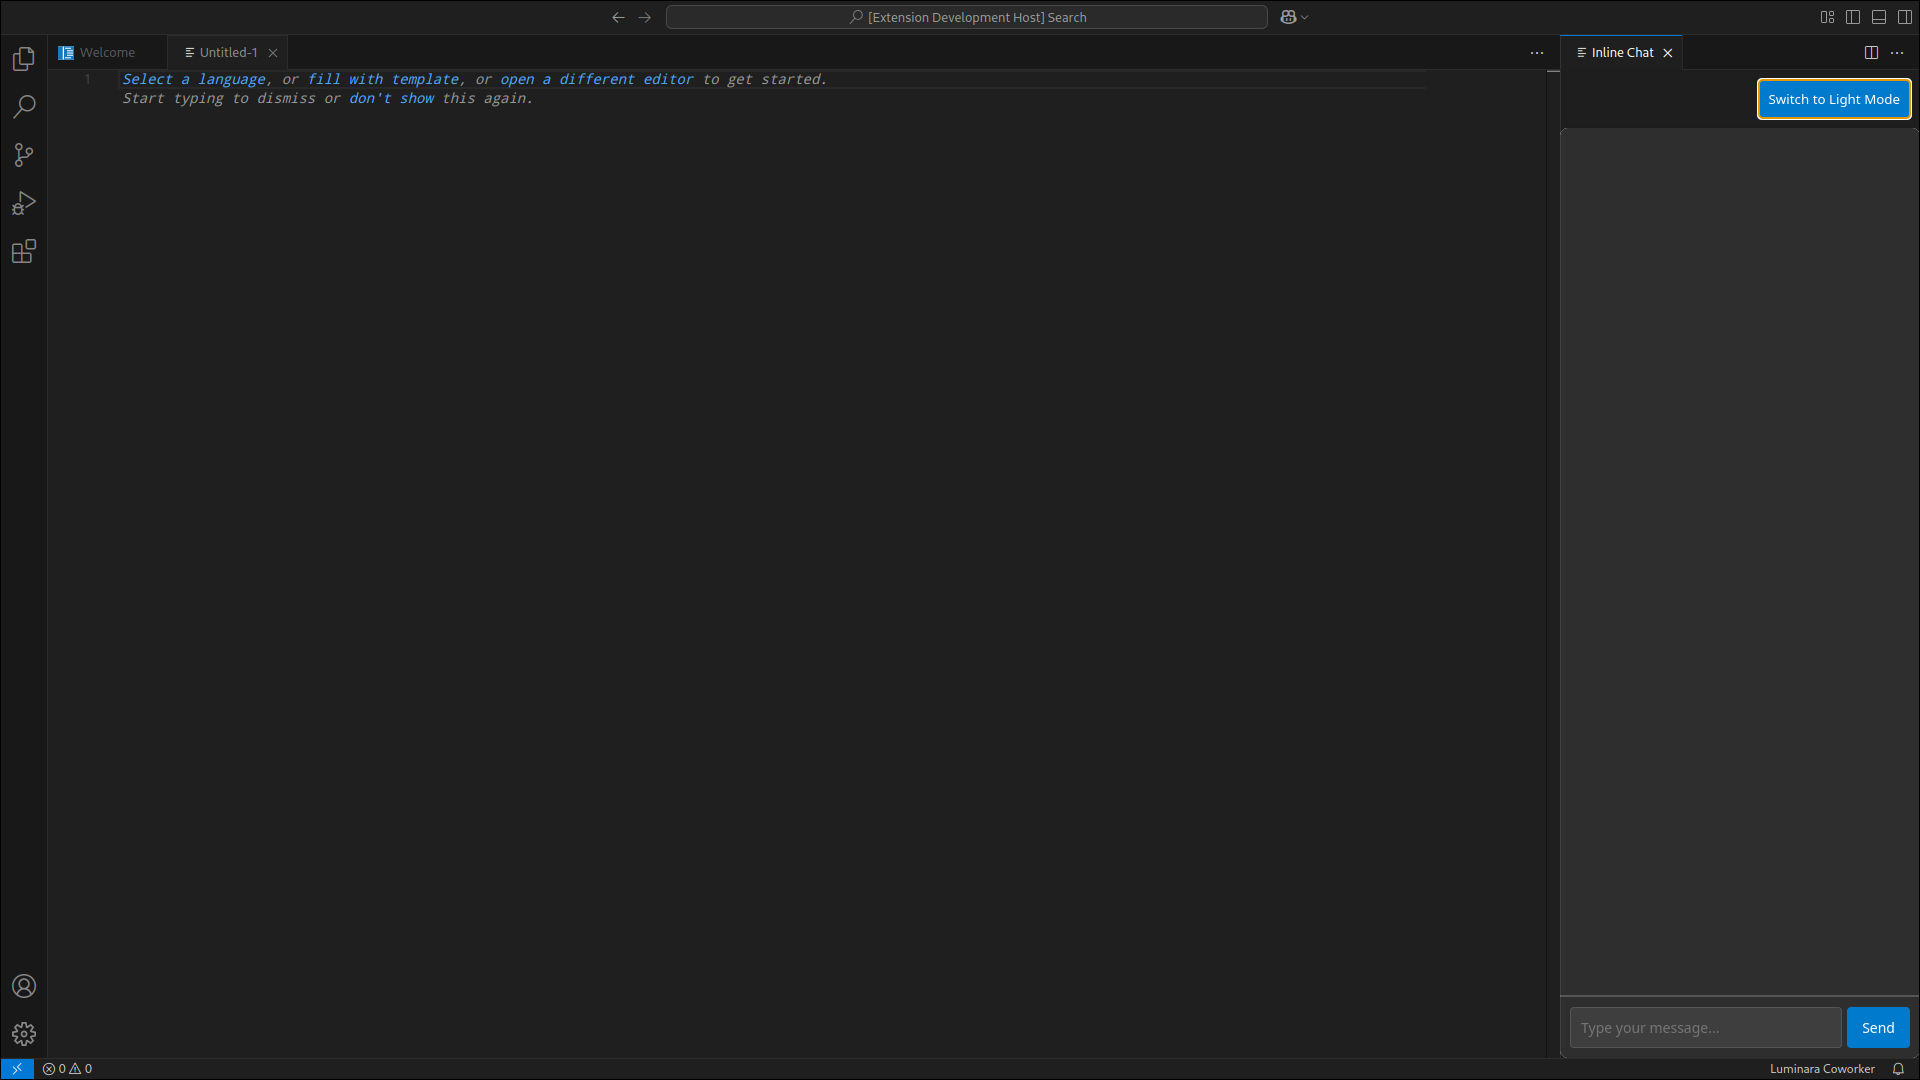
\includegraphics[width=0.8\textwidth]{figures/Extension.png}
  \caption{Extension in VS Code}
  \label{fig:Extension_in_VS_Code}
\end{figure}




\subsection{Chat}

The chat is integrated into the IDE with a webview. 
Webviews are a tool provided by the VS Code API. They can be used to implement various GUIs into the IDE. 

The following code, defines the properties of the Webview an initiates the GUI.

\begin{lstlisting}[language=TypeScript, caption={Create webview}]

    // defining the properties of the webview
    const panel = vscode.window.createWebviewPanel(
        'inlineChat', // Identifier
        'Inline Chat', // Title
        vscode.ViewColumn.Beside, // Position
        {
        enableScripts: true, // Allow JavaScript
        retainContextWhenHidden: true, // Keep the webview state
        }
    );

    //executing the getWebviewContent function to implement the GUI
    panel.webview.html = getWebviewContent();

\end{lstlisting}

The getWebviewContent function defines the HTML and CSS elements of the Webview.
It also defines the interactions for the GUI with the TypeScript code. 

\begin{lstlisting}[language=HTML, caption={IDE Chat GUI}]

    function getWebviewContent(): string {
        return `
          <!DOCTYPE html>
          <html lang="en">
          <head>
            <meta charset="UTF-8">
            <meta name="viewport" content="width=device-width, initial-scale=1.0">
            <title>Inline Chat</title>


            <style>
            <!--Style for the Chatbot -->
            </style>


          </head>
          <body>
            <!--Button to switch between dark and light mode -->
            <button class="mode-switch" id="modeSwitch">Switch to Dark Mode</button>

            <!--Container for the message -->
            <div class="chat-container">
              <div class="messages" id="messages"></div>
              <div class="input-box">
                <input type="text" id="input" placeholder="Type your message..." />
                <button id="send">Send</button>
              </div>
            </div>

            <!--Backend logic for the chat -->
            <script>
              const vscode = acquireVsCodeApi();

              <!--Sends the message and updates the GUI -->
              document.getElementById('send')
              .addEventListener('click', () => {
                const input = document.getElementById('input');
                const message = input.value.trim();
                if (message) {
                  vscode.postMessage({ command: 'sendMessage', text: message });
      
                  <!--Add user message to chat display -->
                  
                  const messagesDiv = document.getElementById('messages');
                  const newMessage = document.createElement('div');
                  newMessage.className = 'message';
                  newMessage.textContent = message;
                  messagesDiv.appendChild(newMessage);
      
                  <!--Scroll to the latest message -->
                  messagesDiv.scrollTop = messagesDiv.scrollHeight;
      
                  input.value = '';
                }
              });
              <!--Logic for dark and lightmode switch -->
              document.getElementById('modeSwitch')
              .addEventListener('click', () => {
                const body = document.body;
                const modeSwitch = document.getElementById('modeSwitch');
      
                if (body.classList.contains('dark-mode')) {
                  body.classList.remove('dark-mode');
                  modeSwitch.textContent = 'Switch to Dark Mode';
                } else {
                  body.classList.add('dark-mode');
                  modeSwitch.textContent = 'Switch to Light Mode';
                }
              });
      
              <!--Handles the display of the reply message -->
              window.addEventListener('message', (event) => {
                const message = event.data;
                if (message.command === 'displayReply') {
                  const messagesDiv = document.getElementById('messages');
                  const newReply = document.createElement('div');
                  newReply.className = 'bot-reply';
                  newReply.textContent = message.text;
                  messagesDiv.appendChild(newReply);
      
                  <!--Scroll to the latest message -->
                  messagesDiv.scrollTop = messagesDiv.scrollHeight;
                }
              });
            </script>
          </body>
          </html>
        `;
\end{lstlisting}



\subsection{Server Request}

After the user clicks send in the chats GUI, the onDidReceiveMessage command is executed.This command initiates the server request.
It also defines the payload that the server receives. The payload contains the question asked, aswell as the baseprompt defined by the developers. 

The request to the server is handled with Axios. Axios sends the respond to one of the Flask Service endpoints that are hosted on the server.
\ref{cha:hosted_flask_service}

After the response reaches the client, the responses text is displayed in the chat GUI. On a failed request an error message is displayed.

\begin{lstlisting}[language=TypeScript, caption={Axios request}]
    // executes when the "send" button is clicked in the GUI
    panel.webview.onDidReceiveMessage(
        async (message) => {
          if (message.command === 'sendMessage') {
            //defines the payload that is sent
            const payload = {
              model: 'qwen2.5-coder:0.5b',
              prompt: message.text
            };  

    try {
        const response = await axios.post('http://10.10.11.11:5001
        /ask_programming_bot', payload ); 
        //Selecting the endpoint for the request and sending the payload. 
        const reply = await response.data.choices[0].text; //the response is then stored in the "reply" variable

        //formating the reply and showing it in the editor
        editor.edit((editBuilder) => {
          reply.split('```').forEach((reply: string) => {
            editBuilder.insert(position, `\n  # ${reply} \n`);
          });
        });

        // Send the reply to the webview to display it
        panel.webview.postMessage({
          command: 'displayReply',
          text: reply.split('```').map((reply: string) => reply)
        });

    //Display and error message on failed request
      } catch (error) {
        vscode.window.showErrorMessage('Failed to get response from the server.');
      }

\end{lstlisting}

\subsection{Status Bar Item} 

The extension also provides a status bar button that can be used to open the chat.

In the following code the Status Bar Item is created and the commands are registered.

\begin{lstlisting}[language=TypeScript, caption={Status Bar}]
  //Creates a status bar item
  const commandId = 'luminara-coworker.statusBarClicked';

  //Registers the command
	context.subscriptions.push(vscode.commands
  .registerCommand(commandId, async () => {
    // Defines the options of the Quick Pick menu
		const pageType = await vscode.window.showQuickPick(
			['Message', 'Chat GPT-04', 'Chat Ollama', 'Inline chat'],
			{ placeHolder: 'select a function' });
\end{lstlisting}

To assign a command it first has to be registered into the extension. This is done at the start of every TypeScript file that defines an command.

\begin{lstlisting}[language=TypeScript, caption={registering Command}]

  export async function createInlineChat(context: vscode.ExtensionContext ) {

  const disposable = vscode.commands
  .registerCommand('luminara_coworker.startInlineChat', () => {
    // Code for the Command
  }
\end{lstlisting}


After registering a command it can be assigned to the status bar. After selecting the command the defined code will be executed.

\begin{lstlisting}[language=TypeScript, caption={assigning Command}]
  if (pageType === 'Inline chat') {
        
    vscode.commands
    .executeCommand("luminara_coworker.startInlineChat");
  }
\end{lstlisting}
    

\subsection{Deploying the Extension}

After programming all the necessary components for the extension, they have to be registered into the extension.ts file.
There they can be assigned to a specific extension context. Only files that are registered in the activate function are deployed when the extension is started.

\begin{lstlisting}[language=TypeScript, caption={Deploying the Extension}]

  export function activate(context: vscode.ExtensionContext) {

	console.log('Congratulations, your extension "luminara-coworker" is now active!');
	
	const disposable = vscode.commands
  .registerCommand('luminara-coworker.helloWorld', () => {
		vscode.window.showInformationMessage('Hello World from luminara_coworker!');
	});
			
	createStatusbarItem(context);
	luminaraChat(context);
	luminaraChatOllama(context);
	createInlineChat(context);



	context.subscriptions.push(disposable);
}
\end{lstlisting}



\section{Conclusion}

The VS Code extension provides a seamless integration of the chatbot functionality into the IDE. By leveraging the VS Code API and Axios, the extension enables users to interact with the chatbot directly within the editor, enhancing the development experience. The extension's core features, such as the chat interface and server request handling, are designed to streamline the user's workflow and provide quick access to AI-powered assistance.